% 11-761 Language and Statistics
% Assignment 3

\pdfoutput=1
\documentclass[11pt]{article}
\usepackage[left=1in,top=1in,right=1in,bottom=1in,nohead,nofoot]{geometry}
\usepackage{amsmath}
\usepackage{amsthm}
\usepackage{hyperref}
\usepackage{verbatim}
\usepackage{float}
\usepackage{graphicx}
\usepackage{longtable}
\usepackage{todonotes}
\usepackage{wrapfig}
\newcommand{\f}[2]{\frac{#1}{#2}}
\newcommand{\ngram}{\mbox{$n$-gram }}
\newcommand{\ngrams}{\mbox{$n$-grams }}

\newcommand{\leocomment}[1]{\todo[color=red!40,caption={Leo's comment}]{#1}}
\newcommand{\hectcomment}[1]{\todo[color=green!40,caption={Hector's comment}]{#1}}
\newcommand{\dicomment}[1]{\todo[color=violet!40,caption={Di's comment}]{#1}}
\newcommand{\zhoucomment}[1]{\todo[color=blue!40,caption={Zhou's comment}]{#1}}

\restylefloat{table}
\restylefloat{figure}

\begin{document}

\title{11-761 Language and Statistics - Spring 2013\\
Course Project}
\author{Leonid (Leo) Boytsov, Zhou Yu, Di Wang, Hector Liu}
\date{}
\maketitle

\begin{abstract}
We took a machine learning approach and trained two discriminative classifiers:
a soft-margin SVM and a regularized logistic regression.
The SVM is used for classification, while the logistic regression is used to produce posterior probabilities.
To reduce the risk of overfitting, we generated additional training and testing data.
\end{abstract}

%\thispagestyle{empty}
%\setlength{\parindent}{0pt}

\section{Introduction}
Our group decided to focus on getting good performance with respect to the ``hard'' metric.
We employed discriminative classifiers,
because they are often superior to generative ones on the classification task. \cite{roni2013,bishop2007generative}.
\footnote{See also \url{http://xiaodong-yu.blogspot.com/2009/10/good-summary-on-generative-vs.html}.}
To reduce the risk of overfitting, we generate additional training data and testing data.
The details are given in subsequent sections. The individual contributions of team members are summarized in Table\ref{TableContrib}.


\begin{table}[H]
\begin{tabular}{p{1in}|p{5in}}
\hline
Leo Boytsov &  Wrote code to produce features based on \ngram models (including models based on POS-tag sequences), generated additional training/testing data, and fine-tuned machine learning models;
\\\hline
Zhou Yu & Implemented and designed code for classification and computation of posterior probabilities;
\\\hline
Di Wang & Tested additional features, in particular, based on word co-occurrences (computed
as mutual information) and carried out an error analysis;
\\\hline
Hector Liu & Helped Leo to generate POS-tag based \ngram models, wrote a
reliable RunMe script that feeds language-model features to machine learning code
and extracts results.
\\\hline
Everybody & Participated in the design process and described his/her work
in the report and the presentation.
\\\hline
\end{tabular}

\caption{\label{TableContrib}Individual contributions of team members.}
\end{table}

\section{Training the Models}
\subsection{Choosing Features} 
Fake documents were generated using a tri-gram model, 
which is based on the histories of depth three.
Hence, we expected that features computed over longer histories would be useful in distinguishing 
between fake and real documents.
In particular, we employed 
perplexities computed using higher order \ngram models ($n>3$).

The \ngram models were created with the help of the CMU-Cambridge toolkit\footnote{\url{http://svr-www.eng.cam.ac.uk/~prc14/toolkit.html}}.  The Broadcast News corpus was used for training.
We employed six \ngram models ($2 \le n \le 7$), which were smoothed using the Good-Touring method.
For $n>2$ the models included only \ngrams that occurred more than once (the larger is $n$, the larger is the cutoff value).

In addition, we tried several other feature types:
\begin{itemize}
\item \ngram models for sequences of POS tags. To this end, we applied the Stanford POS tagger
to the Broadcast News corpus.
\item language models based on word co-occurrences inside and across sentences.  


\item the total number of words in a document and the number of words \texttt{<UNK>}.
\end{itemize}
All these additional features were inferior to perplexities computed from the \ngram models.
In particular, the accuracy of a classifier built on top of the POS-tag-based language models
was less than 70\%. Combining POS-tag-based \ngram models with regular \ngram models did not lead
to better classification accuracy.

\subsection{Generating Additional Training/Testing Data}\label{SectGen}
Because the CMU-Cambridge toolkit cannot generate data from a tri-gram model,
we tried to employ the NLTK tookit (using Broadcast News corpus as a training set).
Unigrams not included in the tri-gram model (provided by instructors) were replaced by the word \texttt{<UNK>}.
Real sentences were randomly sampled from the Broadcast News corpus.
For both real and fake data, document lengths were chosen randomly to mimic distribution in the training data.
Unfortunately, this data proved to be completely useless. The feature values for the generated data
and the training set provided by instructors were substantially different.

Then, we found that the CMU Sphinx toolkit\footnote{\url{http://cmusphinx.sourceforge.net/}}
included a version of the CMU-Cambridge toolkit capable of generating fake texts.
However, we could not make the Sphinx toolkit read the provided binary language model (the \texttt{binlm}-file).\footnote{It complained that the model was corrupt.} Nor did the Sphinx toolkit
support generation from the text version of the language model (the \texttt{arpa}-file).
Hence, we back-ported the generating function to the CMU-Cambridge toolkit.

We also changed an approach to generate real documents.
It appears to us that the Broadcast News corpus contains complete documents, but their boundaries are not marked.
To generate a document containing a desired number of
words, we start from the beginning of a random sentence and select a contiguous sequence
of words. Thus, generated documents contain long pieces of coherent text (with similar statistical properties).
For the reasons explained in section \ref{SectTrain}, on average, a generated document is
2000 words longer than  a document from the provided training set.

\subsection{Choosing and Training the Models}\label{SectTrain}
For the purpose of classification we use a soft-margin SVM with a linear kernel. 
More specifically, we employ the package LIBLINEAR,
which is very efficient and reliable \ref{REF08a}.
To produce posterior probability we train another discriminative model: a
regularized logistic regression.
Two regularization methods were tested: the LASSO and the Tikhonov regularization.
The soft metric cannot be computed, if any probability is zero,
hence, posterior probabilities were smoothed.
Parameters were chosen empirically (with performance evaluated through 10-fold cross-validation).

Additionally, we tested the SVM with the RBF kernel and a continuous Naive Bayes (with the normal kernel).
The RBF-based SVM was overfitting (despite we tried various margin coefficients and kernel widths).
The Naive Bayes also performed badly (for unknown reason).

The observed log-perplexity is an average value taken over log-perplexities of document \mbox{$n$-grams}. 
We adopt a point of view that the log-perplexity is sampled from a random variable
(or a parametric family of random variables).
Thus, the average document log-perplexity is an MLE estimate of this random variable mean.
We argue that performance of machine learning models depend on how
well they learn parameters of this distribution (or distribution families), in particular their mean values.

The shorter is a document, the higher is the variance of the mean estimates
and, consequently, the harder it is for the model to ``guess'' true mean values.
Hence, if a document length (or a number of words)
is not included as a feature,
models could produce better results when they are trained on longer documents.
These documents cannot be excessively long,
because long spans of text in the Broadcast Corpus may contain multiple documents
with very different properties.

In particular, when we train and test on the same DEV set, we get much worse
accuracy, then when we train on the training set and test on the DEV set!
This is somewhat paradoxical, because the DEV set contains mostly short documents (around 100-200 words),
 while the training set contains few or no documents shorter than 100 words.
Thus, one may consider this training set as being not representative.

\begin{table}
\caption{\label{TablePerf}  Performance data for various data and feature sets.}
\begin{tabular}{c|c|c|c|c|c|c|c|c|c|c|c|c|c|c|c}\hline
\multicolumn{8}{c}{\textbf{Original} DEV set} \\\hline\hline
\multicolumn{4}{c|}{SVM performance } & \multicolumn{4}{c}{Logistic regression (LASSO) performance } \\
\multicolumn{4}{c|}{(hard metric)} & \multicolumn{4}{c}{(soft metric/$2^{\mbox{soft metric}}$)} \\\hline\hline
\multicolumn{2}{c|}{Original training set} & \multicolumn{2}{c|}{Generated training set}
&
\multicolumn{2}{c|}{Original training set} & \multicolumn{2}{c}{Generated training set}
\\\hline
short & complete & short & complete  &
short & complete & short & complete  \\
features & features & features & features &
features & features & features & features \\\hline
0.88  & 0.90 & 0.92 &  0.895  & -0.51/0.7 & -0.46/0.73 & -0.41/0.75 & -0.4/0.76

\\\hline
\multicolumn{8}{c}{\textbf{Generated} DEV set} \\\hline\hline
\multicolumn{4}{c|}{SVM performance } & \multicolumn{4}{c}{Logistic regression (LASSO) performance } \\
\multicolumn{4}{c|}{(hard metric)} & \multicolumn{4}{c}{(soft metric/$2^{\mbox{soft metric}}$)} \\\hline\hline
\multicolumn{2}{c|}{Original training set} & \multicolumn{2}{c|}{Generated training set} &
\multicolumn{2}{c|}{Original training set} & \multicolumn{2}{c}{Generated training set} \\\hline
short & complete & short & complete  &
short & complete & short & complete  \\
features & features & features & features &
features & features & features & features \\\hline
0.93 & 0.92   & 0.93 & 0.9  & -0.32/0.8  & -0.36/0.78 & -0.33/0.8 & -0.46/0.73\\\hline
\end{tabular}
\end{table}

\section{Experiments}
In addition, to the training and DEV sets provided by instructors,
we used data generated by our team (see Section \ref{SectGen}).
Our synthetic training and development sets include 10,000 and 2,000 documents, respectively.

We employed two sets of \ngram based features. The complete set includes perplexities for six \ngram models,
but the short set employs only the 3-gram and the 4-gram models.
When we use only the provided training data, it does not hurt to include all features into the SVM
model (see Table~\ref{TablePerf}). As we get more training data, it may be better to use only
the 3-gram and the 4-gram models.

\begin{wrapfigure}{l}{0.45\textwidth}\centering
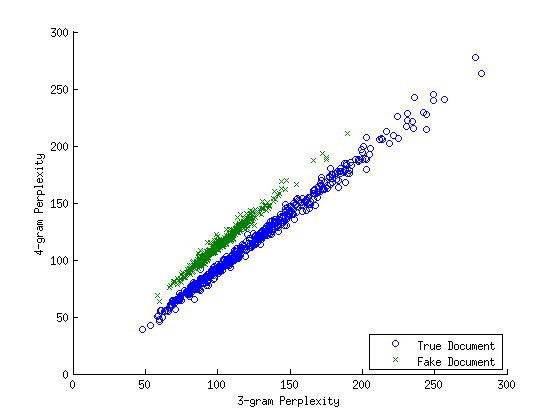
\includegraphics[scale=0.5]{erroranalysisGram34.png}
\caption{Perplexities for 3- and 4-gram models computed for the original \textbf{training} set.\label{Fig1}}
\end{wrapfigure}

As we can see from Figure~\ref{Fig1},
in the training set,
these two models alone separate the fake and real documents almost perfectly.
Note, though, that for a development set, the ``clouds'' of real and fake documents have a considerable overlap.
 As explained in Section \ref{SectGen}, this is due to the fact that the training set
contains only few short documents and, consequently, perplexity values have little variance due to random effects.
Other types of features were less useful in separating fake and real documents. For example,
the point-wise mutual information between distant words is generally different for real and fake documents,
but there is also a large overlap (see Figure~\ref{FigNPMI}). 

We also believe that there may exist a \textbf{latent variable} that determines the complexity
of the document lexicon.
If the document contains a lot of rare words, both the 3-gram and the 4-gram models
would be surprised to see it. In contrast, documents with a lot of common words
have low perplexity values for all \ngram models.
The value of document perplexity with respect to any \ngram model varies considerably
and none of the model is sufficient to detect fake sentences.
Yet, this is possible with two models.

Our classifier performs better on long sentences (see Table~\ref{TableCorr}).
For document containing only one sentence, we can detect fake sentences with $\approx 75\%$ accuracy
for both the original and generated DEV sets.
Exactly half of all documents are fake. Hence, we are doing much
better than random guessing (by flipping a fair coin), which would get correctly only 50\% of documents.
For longer documents, the accuracy is mostly higher than 95\%.
Yet, because documents having 1-2 sentences comprise 30\% of all DEV documents,
it is hard to get the overall accuracy higher than 90\%.

\begin{table}\centering
\caption{Correctness of classification depending on document length\label{TableCorr}}
\begin{tabular}{c|c|c|c|c|c|c|c|c|c}
\# of sentences.  &  1   &  2   &   3   &  4   &   5   &    7  & 10   & 15   &  20  \\\hline
share in DEV set  & 20\% & 10\% &  10\% & 10\% &  10\% &  10\% & 10\% & 10\% & 10\%  \\\hline\hline
Original DEV      & 0.75 & 0.9  &  0.9  & 0.95 & 0.95  &    1  &   1  &   1  &  1 \\\hline
Generated DEV     & 0.73 & 0.86 &  0.86 & 0.91 & 0.95  &   0.96&  0.99 &  1  &  1 \\\hline
\end{tabular}
\end{table}

Unlike the classification task, it is less clear whether the complete set of features is better or worse
than the short set of features for the purpose of producing posterior probabilities.
According to Table~\ref{TablePerf}, the complete set of features performs better with a small training set.
For the generated training set, the complete set of features is better only on the original DEV set,
but it performs worse on the generated DEV set.
Nevertheless, we chose the complete set,
because the generated set was created by us and might have been less representative of the unseen test data.
Note that Table~\ref{TablePerf} includes data only for the LASSO
regularization, because the Tikhonov regularization was somewhat inferior (and is not presented here).

\begin{wrapfigure}{r}{0.45\textwidth}\centering
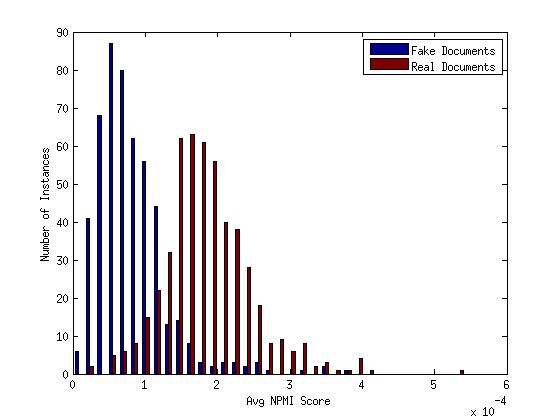
\includegraphics[scale=0.45]{./erroranalysisNPMI.png}
\caption{A distribution of the average Normalized Pointwise Mutual Information (NPMI) 
between distant words computed for the original \textbf{training} set.\label{FigNPMI}}
\end{wrapfigure}

\section{Conclusions}
We took a machine learning approach and trained two discriminative classifiers.
The soft-margin SVM turned to be the best method for the classification task,
while the logistic regression with the LASSO regularization was
the best method to estimate posterior probabilities.
We also found that simple features: perplexities computed from \ngram models were sufficient to achieve good performance.
All other approaches failed to produce better results.
Interestingly enough, no single \ngram model is sufficient to distinguish between real from fake sentences.
Yet, detection is possible and accurate if two models are used (especially the 3-gram and the 4-gram model). 
Additional training data (generated by our team) allowed us to achieve better
results on the DEV set. Yet, the improvement was marginal and might have been due to random effects.

\bibliographystyle{plain}
\bibliography{report}

\end{document}
